\section{Параметрический бутстреп}

Может показаться странным использование бутстреп алгоритма для оценки стандартных ошибок, когда можно использовать формулу из учебника. Фактически, бутстреп выборки могут генерироваться параметрически, в этом случае результаты тесно связаны с формулами стандартных ошибок из учебников. 

Параметрическая бутстреп оценка стандартной ошибки определяется как 
\begin{equation}
    se_{\hat F_{par}}(\hat\theta^*),
\end{equation}
где $\hat F_{par}$ -- оценка $F$, полученная из параметрической модели данных. Здесь мы приведем простой пример, чтобы проиллюстрировать идею. Для данных о юридических школах, вместо оценки $F$ эмпирическим распределением $\hat F$, мы могли бы предположить, что популяция имеет двумерное нормальное распределение. Разумные оценки среднего значения и ковариации этой совокупности даны как $(\bar y, \bar z)$ и
\begin{equation}
    \frac{1}{14}\left(
    \begin{array}{cc}
        \sum(y_i-\bar y)^2 & \sum(y_i-\bar y)(z_i-\bar z) \\
        \sum(y_i-\bar y)(z_i-\bar z) & \sum(z_i-\bar z)^2
    \end{array}
    \right).
\end{equation}
Обозначим двумерную нормальную популяцию с этим средним значением и ковариацией как $\hat F_{norm}$; это пример параметрической оценки совокупности $F$. Используя это, параметрическая бутстреп оценка стандартной ошибки корреляции $\hat\theta$ является $se_{\hat F_{norm}} (\hat\theta^*)$. Как и в непараметрическом случае, идеальная параметрическая бутстреп оценка не может быть легко вычислена, за исключением тех случаев, когда $\hat\theta$ является средним. Поэтому мы аппроксимируем идеальную бутстреп оценку с помощью бутстреп выборок, но другим способом, чем раньше. Вместо выборок с заменой из исходных данных мы берем $B$ выборок размера $n$ из параметрической оценки генеральной совокупности $\hat F_{par}$:
\begin{equation}
    \hat F_{par}\rightarrow(x_1^*,x_2^*,\ldots,x_n^*).
\end{equation}
После генерации бутстреп выборок мы действуем точно так же, как в шагах 2 и 3 бутстреп алгоритма из раздела 6.2: мы оцениваем нашу статистику для каждой бутстреп выборки, а затем вычисляем стандартное отклонение $B$ бутстреп репликаций.

В примере с коэффициентом корреляции, предполагая двумерную нормальную совокупность, мы берем $B$ выборок размером $15$ из $\hat F_{norm}$ и вычисляем коэффициент корреляции для каждой бутстреп выборки. На левой панели рисунка 6.3 показана гистограмма для $B = 3200$ бутстреп репликаций, полученных таким образом. Это очень похоже на гистограммы на рисунке 6.2. Параметрическая бутстреп оценка стандартной ошибки для этих повторений была $0.124$, что близко к значению $0.131$, полученному на непараметрических бутстреп выборках.

Учебная формула для стандартной ошибки коэффициента корреляции составляет $(1-\hat\theta^2) / \sqrt{n- 3}$. Подставляя $\hat\theta = 0.776$, она дает значение $0.15$ для данных о юридических школах.
\newline

\noindent
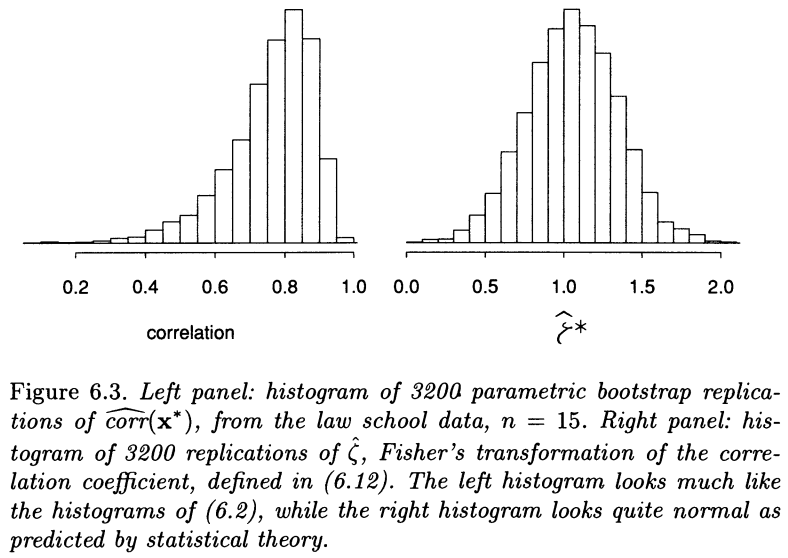
\includegraphics[width=\linewidth]{5/f63.png}
\newline
Мы можем провести дальнейшее сравнение с нашим параметрическим бутстреп результатом. Учебные материалы также утверждают, что преобразование Фишера, примененное к $\hat\theta$
\begin{equation}
    \hat\zeta=0.5\log\left(\frac{1+\hat\theta}{1-\hat\theta}\right)
\end{equation}
приблизительно нормально распределено со средним $\zeta= 0.5  \log\left(\frac{1+\theta}{1-\theta}\right)$ и стандартным отклонением $1 / \sqrt{n-3}$, где $\theta$ является коэффициентом корреляции совокупности. Исходя из этого, обычно выполняется вывод для $\zeta$ и затем преобразуется обратно, чтобы сделать вывод о коэффициенте корреляции. Чтобы сравнить это с нашим параметрическим бутстреп анализом, мы вычислили $\hat\zeta$ вместо $\hat\theta$ для каждой из наших $3200$ бутстреп выборок. Гистограмма значений $\hat\zeta^*$ показана на правой панели рисунка 6.3 и выглядит вполне нормально. Кроме того, стандартное отклонение $3200$ значений $\hat\zeta^*$ было $0.290$, что очень близко к значению $1 / \sqrt{15-3} = 0.289$. 

Это соглашение выполняется в целом. Большинство формул для стандартных ошибок в учебниках являются приближениями, основанными на нормальной теории, и обычно дают ответы, близкие к параметрическому бутстрепу, который отбирает выборки из нормального распределения. Взаимосвязь между бутстрепом и традиционной статистической теорией -- более сложная математическая тема.

У бутстрепа есть два несколько отличных друг от друга преимущества по сравнению с традиционными методами из учебников: 1) при использовании в непараметрическом режиме он избавляет аналитика от необходимости делать параметрические предположения о форме базовой совокупности, и 2) при использовании в параметрическом режиме он обеспечивает болле точные ответы, чем формулы из учебника, и могут дать ответы на задачи, для которых не существует формул из учебника. 

Большая часть этого пособия сосредоточена на непараметрическом применении бутстрепа. Параметрический бутстреп полезен в задачах, где доступны некоторые знания о форме генеральной совокупности, а также для сравнение с непараметрическим анализом. Однако основная причина использования параметрических допущений в традиционном статистическом анализе состоит в том, чтобы облегчить вывод формул для стандартных ошибок из учебников. Поскольку нам не нужны формулы в бутстреп подходе, мы можем избежать ограничительных параметрических предположений. 
